\chapter{Human Memory and Learning}
\label{chap:modeling_memory}

Humans learn so that they can get a better fit to the environment: understanding and learning allow for better perception. This Chapter provides an overview on different theories of human learning and memorization. 

\section{Learning and prediction}
Learning theory  advances by quantifying neurobiological \textbf{responses to stimuli} with different levels of probability/stimulus-features. Learning optimizes perception and behavior, with \textbf{surprise} (sometimes called \textit{prediction error}) being a long-considered key component because it is \textbf{a clue to what people know}. Surprise can be measured through different means: physiologically (e.g. pupil dilation), via brain data, and others.
But the S-R (Stimulus-Response) approach depends on more than what people know: it is mediated by low-level perception, accumulation of evidence, report biases, and response-initiation processes (noise). Therefore studying the observed responses to stimuli might not be the best way to understand what people learn.
Moreover, S-R also ignores the issue of whether people use learning to construct \textbf{expectations or predictions}. Computer models do not exhibit this problem, but humans do. Actually, there is no guarantee that our behaviour depends on predictions: it might be that no anticipatory prediction is done before the stimulus is presented; there is huge debate on this topic.
Studies of expectation probe the state of a cognitive system prior to stimulus presentation and independent of stimulus-guided responses. We can measure the expectation of a distribution using the Shannon Entropy. This is related to the surprise to a sample from the distribution. If the sample differs much from the expectation, then the surprise is higher (the subject is learning).

We can use surprise to understand if a person has learned something (surprise means he/she has picked up a distribution): we can observe surprise with respect to event transitions (Markov matrix). We can further observe if a person has just learned the marginal probabilities (how much an event is frequent) or also the conditional probabilities (how frequent an event is after a given other event).

\subsection{Cashdollar et al. (2016)}
They show how \textbf{learning produces predictions}, and \textbf{predictions impact processing}. In particular, they manipulate the randomness of an environment and observe, through MEG, how people behave. Image categories are presented \textbf{randomly} (\texttt{Rand}) or \textbf{predictably} (\texttt{Ord\_75}). Figure \ref{fig:cashdollar} shows that pre-stimulus activity is positively correlated with \textit{Working Memory Capacity} (WMC). \textit{Theta} and \textit{alpha} frequencies effects are observed to understand what happens in the brain. The strength (amplitude) of \textit{theta} oscillations gives a measure of how much the memory activity is involved.

\begin{figure}[!ht]
    \centering
    \captionsetup{width=.8\linewidth}
    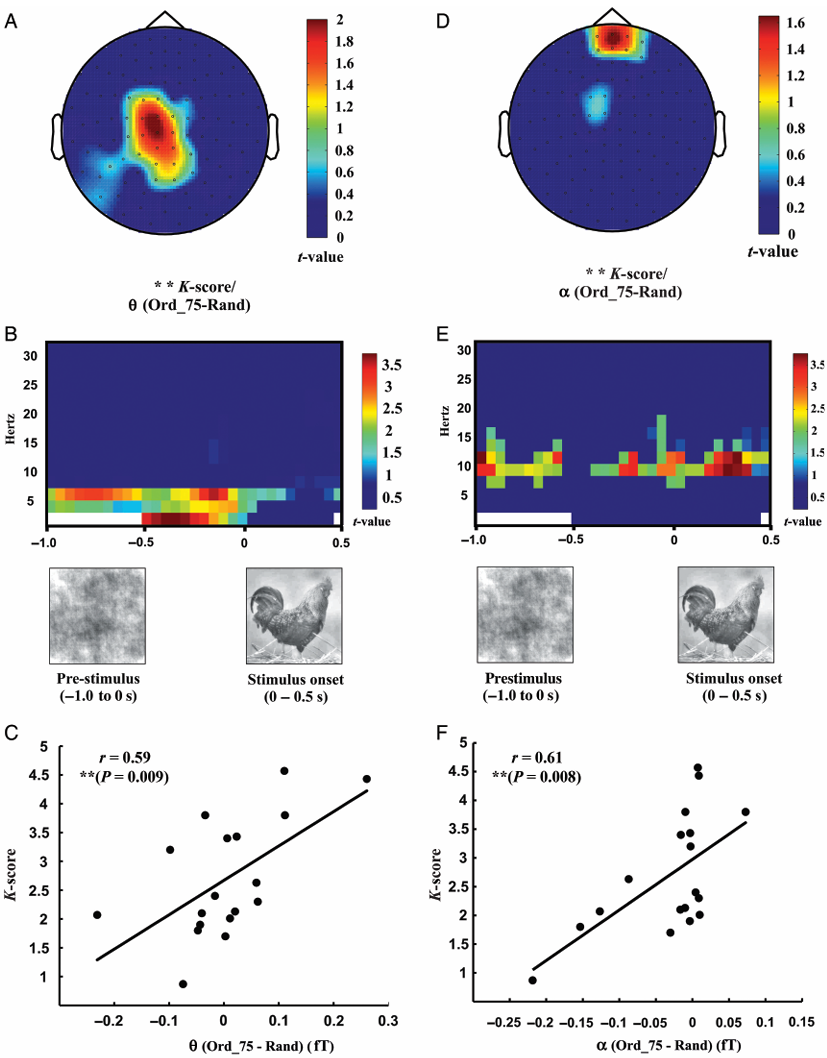
\includegraphics[width=0.75\linewidth]{images/cashdollar.png}
    \caption{Pre-stimulus oscillations and WMC (time 0 is when the next image is presented). Specifically, \textbf{(A)} pre-stimulus power differences in the $\theta$ band (4-8 Hz) between \texttt{Ord\_75} and \texttt{Rand} trials positively correlate with individuals' K-scores within a cluster of central sensors \textbf{(C)} and continue throughout the entire pre-stimulus period but terminates with the onset of the stimulus \textbf{(B)}. Similarly, within a cluster of frontal sensors \textbf{(D)} pre-stimulus power differences in the $\alpha$ band (8–12 Hz) between \texttt{Ord\_75} and \texttt{Rand} trials also positively correlate with individual's K-scores \textbf{(F)}, yet this pattern continues throughout stimulus presentation \textbf{(E)}.}
    \label{fig:cashdollar}
\end{figure}

They also measure how pre-stimulus activity (as a function of regularity \notet) relates to post-stimulus activity. They observe  stronger activity for predictable stimulus ($\text{\texttt{Ord\_75}}-\text{\texttt{Rand}}$, Fig. \ref{fig:cashdollar_2}) for people more sensitive to series order (greater pre-stimulus $\theta$ band power for ordered~vs.~random series). In other words, people who make predictions (those who have learned the distributions, i.e., that have higher post-stimulus activity) are also those having higher pre-stimulus activity.

\osst{As a function of regularity because they manipulate the degree of predictability (i.e., regularity) of the environment.}

\begin{figure}[!ht]
    \centering
    \captionsetup{width=.8\linewidth}
    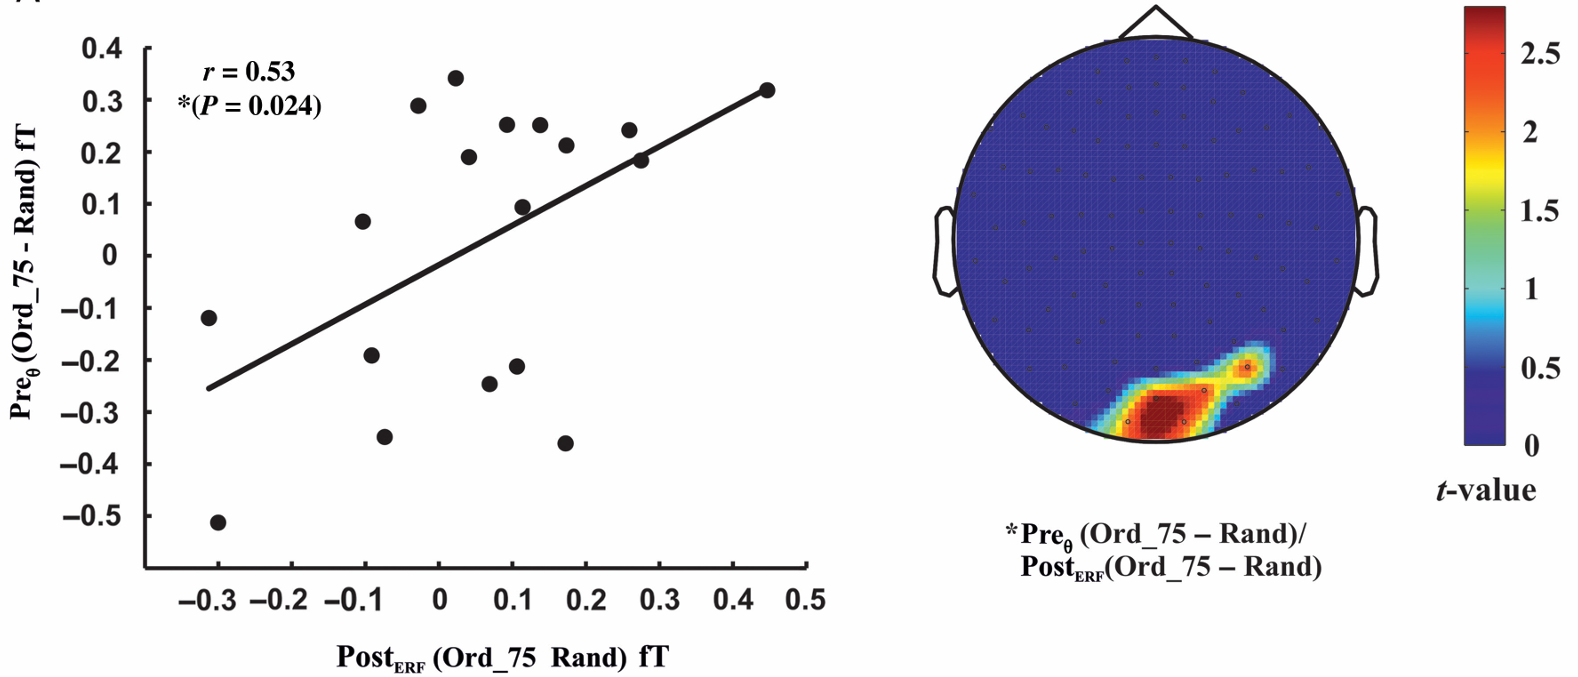
\includegraphics[width=0.7\linewidth]{images/cashdollar_2.png}
    \caption{Pre-stimulus oscillations and post-stimulus neural responses. For each participant, they identified the sensor with the largest absolute pre-stimulus power difference ($\text{\texttt{Ord\_75}}-\text{\texttt{Rand}}$), within the $\theta$ (Pre$_\theta$) and $\alpha$ (Pre$_\alpha$) frequency bands separately (-1.0 to 0 s prior to stimulus onset).}
    \label{fig:cashdollar_2}
\end{figure}

\subsection{The logic of studying learning and prediction}
We need to quantify learning from observable behavior, to separate predictive processes from responses, and to quantify the relation between the two. To this end, in the following we consider \cite{notaro}, a study showing how \textbf{anticipatory fixation offsets carry more information about environmental statistics than reactive stimulus-responses}.

\section[Predictions as a window into learning]{\textit{Predictions as a window into learning}\\ \mandatory{notaro}}
They experiment with 21 volunteers. The person is looking at a screen (in the center). A target symbol is be presented on the right or on the left side of the screen. A Markov process determines the probability of the next target to be on the same side of the previous. If the probability is 70\% we call this \texttt{pret70}, if it is 30\% then \texttt{pret30} (``pret" stands for ``probability of return"). So in \texttt{pret70} the person (if they learn the pattern) should expect the next target to stay on the same side; while in \texttt{pret30} should expect it to change side.

\begin{figure}[!ht]
    \centering
    \captionsetup{width=.8\linewidth}
    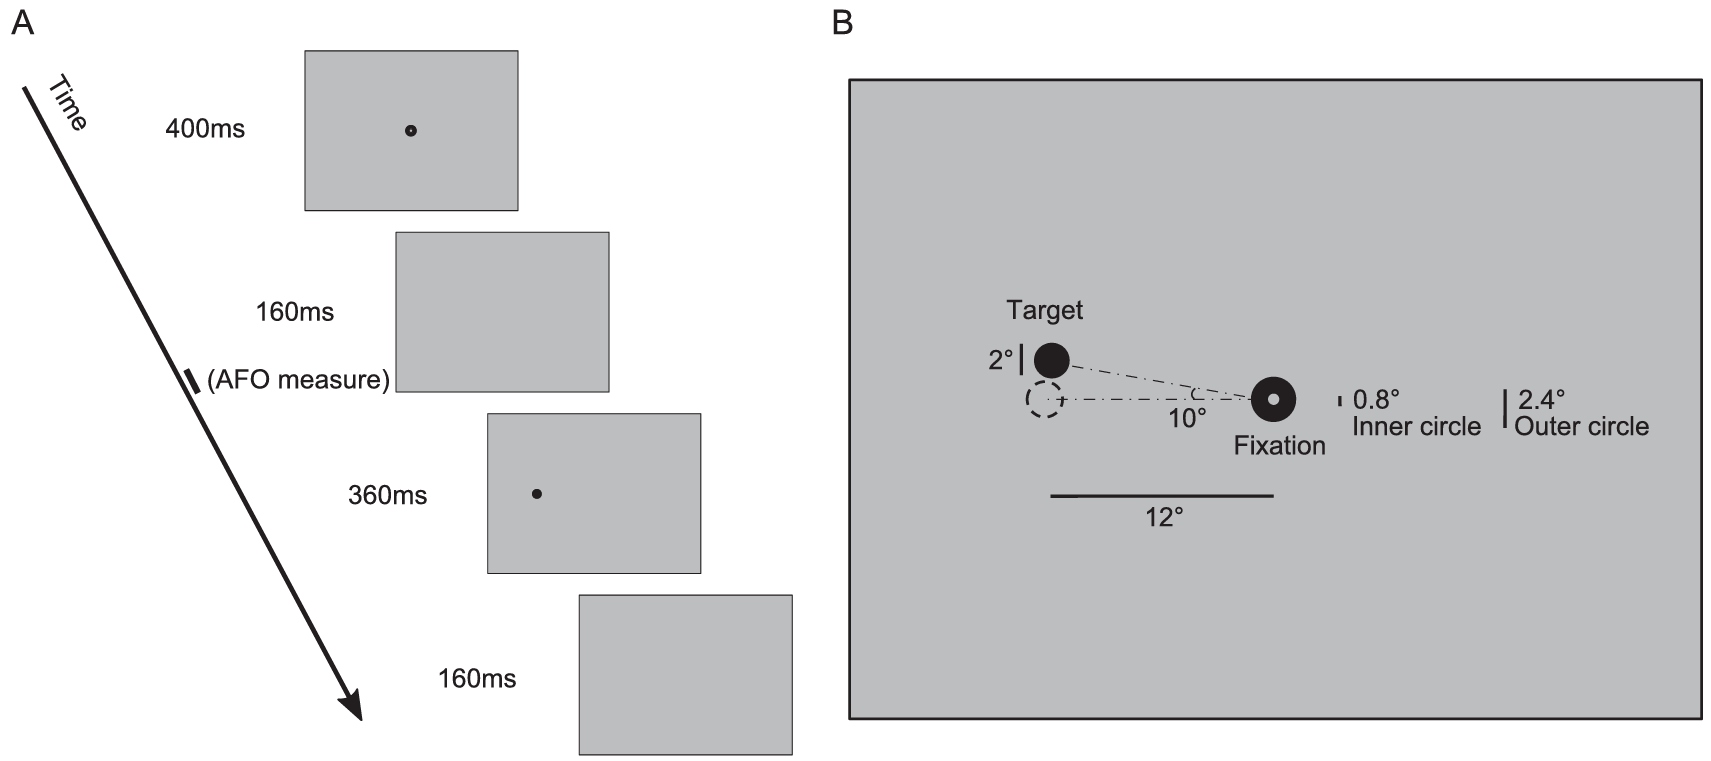
\includegraphics[width=0.7\linewidth]{images/notaro.png}
    \caption{Trial structure and fixation locations. \textbf{(A)} Trial timing. \textbf{\textit{Anticipatory fixation offset}} (\textbf{AFO}) is defined at the mean gaze location during the last 10 ms of the blank screen that followed the fixation symbol and that preceded the target. AFO is coded as positive if to the side of the last target, negative otherwise. \textbf{(B)} Spatial features of fixation and targets. Targets are positioned on an invisible arc that extended 108 above and below the fixation symbol, at 128 eccentricity. The exact location on the arc is randomly set on each trial. The fixation symbol consists of an inner gray circle ($\text{radius} = 0.4\degree$) within an outer black circle ($\text{radius} = 1.2\degree)$.}
    \label{fig:notaro}
\end{figure}

10 series are presented in each condition, each one consisting in 100 trials (Figure \ref{fig:notaro}A shows what a single trial looks like).
The proportion of presentations on the left and right screen sides is 50\% in both conditions (the marginal probability is the same).
Moreover, 20 random-location trials are appended to each series to study wash-out effects. They use an eye-tracking system at 1000 Hz to capture the gaze.
